%% ============================================================
%%  Capitolo 2 – Flusso di Lavoro Digitale e Controllo Qualità
%%  Dispensa del Corso di Patologia Post-Laurea
%%  Questo file è incluso con \input{} da main.tex; NON aggiungere il preambolo qui.
%% ============================================================

\chapter{Flusso di Lavoro Digitale e Controllo Qualità}
\label{ch:2}

% ─────────────────────────────────────────────────────────────
\section{Introduzione}
\label{sec:ch2-intro}

La transizione dalla microscopia ottica convenzionale all'imaging di vetrini interi (WSI) ha
modificato in modo sostanziale la pratica della patologia diagnostica. Anziché un singolo
patologo che esamina un vetrino al microscopio da banco, il moderno laboratorio di patologia
digitale genera immagini digitali ad alta risoluzione che possono essere archiviate, trasmesse e
analizzate computazionalmente. Questo cambiamento introduce sia straordinarie opportunità sia
nuove categorie di rischio. Una diagnosi errata derivante da una scansione sfocata, da una
sezione mal colorata o da un campione mal etichettato non è meno grave di una diagnosi errata su
un vetrino tradizionale; nel dominio digitale, tuttavia, tali errori possono propagarsi
silenziosamente attraverso un intero lotto di casi prima di essere rilevati. Il controllo qualità
(CQ) non è quindi un complemento facoltativo della patologia digitale --- è la disciplina
fondamentale che rende l'intera attività clinicamente sicura e scientificamente riproducibile
\cite{bankhead2022}.

Il flusso di lavoro della patologia digitale può essere concettualizzato come una pipeline lineare
con diverse fasi discrete: ricezione del campione e descrizione macroscopica, processazione
tissutale e preparazione del vetrino, scansione, CQ dell'immagine, gestione delle immagini e,
infine, refertazione diagnostica o analisi computazionale. Ogni fase introduce potenziali fonti
di variabilità ed errore. I fattori pre-analitici --- le condizioni in cui il tessuto viene
fissato, processato, sezionato e colorato --- esercitano la maggiore influenza sulla qualità
finale dell'immagine, eppure sono spesso i meno suscettibili di correzione automatizzata. I
fattori post-analitici, come la deriva della calibrazione dello scanner e le differenze di resa
cromatica tra dispositivi, possono essere affrontati computazionalmente, ma solo se vengono prima
identificati attraverso procedure sistematiche di CQ.

Per gli specializzandi in patologia, una comprensione approfondita del flusso di lavoro digitale
è essenziale per due ragioni. In primo luogo, come futuri patologi diagnostici, saranno
responsabili dell'accettazione o del rifiuto delle immagini digitali come idonee alla diagnosi, e
devono essere in grado di articolare le basi tecniche di tale giudizio. In secondo luogo, con il
progredire del campo verso la diagnosi assistita dall'intelligenza artificiale (IA), la qualità
dei dati di addestramento è direttamente determinata dalla qualità dei vetrini e delle scansioni
sottostanti. \emph{Spazzatura in entrata, spazzatura in uscita} non è solo un aforisma
informatico; nella patologia computazionale è un principio di governance clinica. Le sezioni
seguenti ripercorrono il flusso di lavoro digitale dalla ricezione del campione all'immagine
archiviata, con particolare enfasi sui punti di controllo qualità che salvaguardano l'integrità
diagnostica in ogni fase.

L'importanza di un solido sistema di CQ è sottolineata dal crescente corpus di evidenze che
collega la qualità dell'immagine all'accuratezza diagnostica e alle prestazioni dei modelli di
IA. Studi hanno dimostrato che anche una lieve degradazione della messa a fuoco --- impercettibile
all'osservatore umano in un'ispezione superficiale --- può ridurre significativamente la
sensibilità degli algoritmi di apprendimento profondo per il rilevamento e la classificazione dei
tumori \cite{bankhead2022}. Un approccio sistematico alla gestione della qualità, integrato nelle
procedure operative standard del laboratorio e supportato da tecnologie appropriate, è quindi un
prerequisito per qualsiasi servizio di patologia digitale che aspiri all'eccellenza clinica o
scientifica.

% ─────────────────────────────────────────────────────────────
\section{Fase Pre-analitica: Preparazione del Campione e Protocolli di Scansione}
\label{sec:ch2-preanalytical}

\subsection{Fissazione e Processazione Tissutale}

La fissazione adeguata è il singolo fattore determinante più importante della qualità istologica.
Il fissativo standard in anatomia patologica chirurgica è la formalina neutra tamponata al 10\%
(FNT), una soluzione di formaldeide al 3,7--4\% in soluzione salina tamponata con fosfati a
pH~7,0. La formalina reticola le proteine attraverso ponti metilenici, preservando l'architettura
cellulare e prevenendo l'autolisi. Il tempo di fissazione raccomandato per la maggior parte dei
campioni chirurgici è di 6--72 ore; la sotto-fissazione porta a scarso dettaglio nucleare e a
immunoistochimica (IIC) inaffidabile, mentre la sovra-fissazione causa una reticolazione eccessiva
che può mascherare gli epitopi antigenici e ridurre la sensibilità dei saggi molecolari. Per le
biopsie con ago-cannula, il College of American Pathologists (CAP) e il Royal College of
Pathologists (RCPath) raccomandano generalmente un minimo di 6 ore e un massimo di 48 ore.

Dopo la fissazione, il tessuto viene disidratato attraverso una serie graduata di alcoli (70\%,
95\%, 100\%), chiarificato in xilene o in un sostituto dello xilene, e infiltrato con paraffina
fusa sotto vuoto. Questo processo, eseguito in un processore tissutale automatizzato nell'arco di
8--12 ore, rende il tessuto sufficientemente rigido per il sezionamento sottile. La qualità della
processazione dipende in modo critico dalla completezza della disidratazione; l'acqua residua nel
blocco tissutale causa una scarsa infiltrazione della paraffina, con conseguenti sezioni che si
sbriciolano o si lacerano durante la microtomia. L'inclusione --- l'orientamento del tessuto
processato in uno stampo di paraffina fresca --- richiede competenza tecnica, poiché il piano di
sezione deve essere scelto per massimizzare le informazioni diagnostiche. Un orientamento errato
è un errore pre-analitico che non può essere corretto in nessuna fase successiva.

La scelta del programma del processatore tissutale è una variabile di qualità importante. I
programmi di processazione rapida, che utilizzano temperature elevate ed energia a microonde per
accelerare la disidratazione e l'infiltrazione, possono ridurre il tempo di processazione da 12
ore a sole 2 ore. Tuttavia, la processazione rapida può compromettere la morfologia tissutale se
non viene attentamente validata, in particolare per i tessuti adiposi e i campioni di grandi
dimensioni. I laboratori devono validare i propri programmi di processazione per ciascun tipo di
tessuto e monitorare la qualità della processazione attraverso una valutazione regolare della
qualità delle sezioni e delle prestazioni dell'IIC.

\subsection{Sezionamento, Colorazione e Vetrino Coprioggetto}

La microtomia è il processo di taglio di sezioni sottili (tipicamente 3--5~\textmu m) dal blocco
di paraffina mediante un microtomo rotativo. Lo spessore della sezione è una variabile critica:
le sezioni troppo spesse producono nuclei sovrapposti e scarso dettaglio della cromatina, mentre
le sezioni troppo sottili possono non contenere tessuto sufficiente per la diagnosi. Le sezioni
vengono distese su un bagno d'acqua tiepida per eliminare le pieghe, montate su vetrini di vetro
a carica positiva e asciugate in forno a 60\textdegree C per favorire l'adesione. Le macchine
coprivetri automatizzate applicano uno strato sottile di mezzo di montaggio e un vetrino
coprioggetto; la qualità del coprioggetto influisce direttamente sulla qualità della scansione,
poiché le bolle d'aria o lo spessore non uniforme del mezzo di montaggio creano artefatti ottici
che degradano la messa a fuoco.

La colorazione con ematossilina ed eosina (E\&E) rimane il cardine della diagnosi istopatologica.
L'ematossilina, un colorante basico, colora gli acidi nucleici di blu-viola; l'eosina, un
colorante acido, colora le proteine citoplasmatiche e la matrice extracellulare di rosa. Il
preciso equilibrio tra questi due coloranti --- il rapporto E\&E --- varia tra i laboratori e
persino tra lotti di reagenti, producendo la variabilità di colorazione inter-laboratorio che
rappresenta una sfida importante per la patologia computazionale. La colorazione IIC utilizza
anticorpi coniugati a enzimi o fluorofori per rilevare proteine specifiche nelle sezioni tissutali.
I protocolli IIC sono altamente sensibili alle variabili pre-analitiche: il recupero antigenico
(indotto dal calore o enzimatico), la concentrazione dell'anticorpo, il tempo di incubazione e il
sistema di rivelazione influenzano tutti l'intensità finale della colorazione e il fondo. Le
piattaforme di colorazione automatizzata (ad es., Leica BOND, Ventana BenchMark) migliorano la
riproducibilità ma non eliminano la variabilità inter-corsa.

Il coprioggetto è l'ultima fase della preparazione del vetrino ed è spesso sottovalutato come
fonte di problemi di qualità. Il mezzo di montaggio deve essere applicato in quantità sufficiente
a riempire lo spazio tra il tessuto e il coprioggetto senza traboccare, e il coprioggetto deve
essere applicato senza intrappolare bolle d'aria. I coprivetri automatizzati riducono il rischio
di intrappolamento di bolle d'aria ma richiedono manutenzione e calibrazione regolari. L'indice
di rifrazione del mezzo di montaggio deve corrispondere a quello del vetrino coprioggetto
(circa 1,515) per minimizzare le aberrazioni ottiche; l'uso di un mezzo di montaggio errato può
produrre un alone o un effetto shimmer nell'immagine scansionata che degrada la qualità della
messa a fuoco.

\subsection{Preparazione del Vetrino per la Scansione}

Prima che un vetrino venga caricato in uno scanner per vetrini interi, deve soddisfare determinati
criteri fisici. Il vetrino deve essere pulito e privo di polvere, impronte digitali e mezzo di
montaggio residuo sulla superficie del vetro. I codici a barre o i codici QR stampati
sull'etichetta del vetrino devono essere leggibili dal lettore di etichette dello scanner; le
etichette illeggibili sono una causa comune di errori di identificazione del campione. I vetrini
con spessore tissutale eccessivo, bordi del coprioggetto sollevati o coprioggetti rotti possono
inceppare il meccanismo di trasporto del vetrino dello scanner o produrre errori di messa a fuoco.
Un'ispezione visiva pre-scansione da parte del tecnico di laboratorio è quindi un passaggio
essenziale di CQ che deve essere eseguito sistematicamente utilizzando una lista di controllo
standardizzata.

\subsection{Parametri di Scansione}

Gli scanner per vetrini interi digitalizzano i vetrini istologici acquisendo un mosaico di
tessere di immagine sovrapposte che vengono successivamente unite in un'unica immagine di grandi
dimensioni. I parametri di scansione principali sono:

\begin{itemize}
    \item \textbf{Ingrandimento (obiettivo):} La maggior parte degli scanner offre obiettivi
    20$\times$ e 40$\times$, corrispondenti a dimensioni del pixel di circa 0,5~\textmu m e
    0,25~\textmu m rispettivamente. La scelta dell'ingrandimento dipende dal compito diagnostico;
    il 20$\times$ è sufficiente per la maggior parte dell'istologia di routine, mentre il
    40$\times$ è preferito per la citologia e il dettaglio nucleare fine.

    \item \textbf{Qualità della messa a fuoco:} Gli scanner utilizzano algoritmi di messa a fuoco
    automatica per mantenere la messa a fuoco sull'intera superficie del vetrino. La maggior parte
    dei sistemi esegue una mappa di messa a fuoco pre-scansione, campionando i punti di messa a
    fuoco a intervalli regolari sul tessuto, e poi interpola i valori di messa a fuoco tra i punti
    campionati durante la scansione principale. Il tessuto con spessore non uniforme, pieghe o
    bolle d'aria può vanificare l'algoritmo di messa a fuoco automatica, producendo regioni
    sfocate nell'immagine finale.

    \item \textbf{Velocità di scansione:} Velocità di scansione più elevate riducono i tempi di
    elaborazione ma possono compromettere la qualità dell'immagine, in particolare in termini di
    precisione della messa a fuoco e di unione delle tessere. I laboratori devono validare la
    relazione tra velocità di scansione e qualità dell'immagine per il loro specifico modello di
    scanner e i tipi di tessuto.

    \item \textbf{Z-stacking:} Alcuni scanner possono acquisire più piani focali (z-stack) a
    diverse profondità all'interno della sezione tissutale, producendo un dataset tridimensionale
    da cui è possibile calcolare un'immagine a profondità di campo estesa. Lo z-stacking è
    particolarmente utile per i preparati citologici, dove le cellule a diverse profondità
    potrebbero altrimenti risultare sfocate, ma aumenta sostanzialmente il tempo di scansione e
    le dimensioni del file.
\end{itemize}

La calibrazione dello scanner --- inclusi il bilanciamento del bianco, l'uniformità
dell'illuminazione e il profilo colore --- deve essere eseguita regolarmente secondo il programma
del produttore e verificata con vetrini di riferimento. La deriva della calibrazione è una fonte
sottile ma importante di variabilità cromatica inter-scansione che può confondere sia
l'interpretazione umana sia gli algoritmi di IA \cite{bankhead2022}. I laboratori devono
mantenere un registro degli eventi di calibrazione dello scanner e monitorare lo stato della
calibrazione come parte del loro programma di CQ di routine.

% ─────────────────────────────────────────────────────────────
\section{Strategie di Campionamento e Descrizione Macroscopica}
\label{sec:ch2-sampling}

\subsection{Descrizione Macroscopica}

L'esame macroscopico è il primo passaggio analitico eseguito dal patologo o dall'assistente di
patologia alla ricezione di un campione chirurgico. Una descrizione macroscopica sistematica
documenta il tipo di campione, le dimensioni, il peso, le caratteristiche della superficie esterna
e l'aspetto della superficie di taglio. Per i campioni oncologici, la descrizione deve includere
le dimensioni del tumore, la localizzazione, la distanza dai margini chirurgici e la presenza di
linfonodi o altre strutture anatomiche. Queste informazioni non sono meramente amministrative;
guidano direttamente la selezione dei blocchi tissutali per l'esame istologico e determinano se
il campionamento è adeguato per la stadiazione e la valutazione dei margini.

La descrizione macroscopica deve seguire un modulo standardizzato appropriato al tipo di campione.
I moduli standardizzati, come quelli pubblicati dal Royal College of Pathologists o dal College
of American Pathologists, garantiscono che tutte le caratteristiche diagnosticamente rilevanti
siano registrate e che la descrizione sia riproducibile tra osservatori diversi. Nel contesto
della patologia digitale, le immagini macroscopiche --- fotografie della superficie di taglio del
campione --- sono sempre più incorporate nel fascicolo digitale del caso, fornendo un riferimento
visivo che integra le immagini microscopiche e facilita la correlazione tra i reperti macroscopici
e microscopici.

La documentazione dei reperti macroscopici nell'era della patologia digitale va oltre la
descrizione scritta. La fotografia macroscopica, con fotocamere calibrate e carte di riferimento
cromatico, fornisce una documentazione visiva permanente del campione che può essere esaminata
insieme alle immagini microscopiche. Alcuni laboratori stanno iniziando a esplorare la scansione
tridimensionale dei campioni macroscopici mediante luce strutturata o tomografia computerizzata,
che potrebbe fornire un riferimento volumetrico per il campionamento microscopico.

\subsection{Strategie di Campionamento per Diversi Tipi di Campione}

\paragraph{Biopsie con ago-cannula.}
Le biopsie con ago-cannula sono piccoli cilindri tissutali, tipicamente lunghi 1--2~cm e con un
diametro di 1--2~mm, ottenuti mediante biopsia percutanea con ago di organi solidi (mammella,
prostata, rene, fegato). Poiché il volume tissutale è limitato, tutti i cilindri vengono
solitamente inviati per l'esame istologico. I cilindri vengono inclusi in un unico blocco e si
tagliano più livelli (tipicamente 3--5) per massimizzare la probabilità di campionare la lesione.
Nel flusso di lavoro digitale, la piccola area tissutale significa che la scansione a 20$\times$
è solitamente sufficiente e i tempi di scansione sono brevi.

\paragraph{Campioni da escissione e resezione.}
I campioni da resezione (ad es., colectomia, mastectomia, nefrectomia) sono di grandi dimensioni
e richiedono un campionamento selettivo. Il patologo deve identificare le aree diagnosticamente
più informative --- il centro del tumore, il fronte invasivo, i margini chirurgici e le aree
macroscopicamente anomale --- e inviare blocchi rappresentativi. I protocolli di campionamento
sono definiti da linee guida nazionali e internazionali e devono essere documentati nella
descrizione macroscopica. Il sotto-campionamento è una fonte significativa di errore diagnostico;
ad esempio, il mancato campionamento del punto più profondo di un tumore colorettale può portare
a una sottostadiazione della categoria T.

\paragraph{Campioni citologici.}
I preparati citologici --- inclusi gli strisci da agoaspirato con ago sottile (FNAC), i preparati
citologici in fase liquida (LBC) e i campioni di espettorato o urina --- presentano sfide di
campionamento uniche. La cellularità del preparato è molto variabile e le cellule diagnostiche
possono essere scarsamente distribuite. Nel flusso di lavoro digitale, i vetrini citologici
vengono tipicamente scansionati a 40$\times$ per catturare il dettaglio nucleare fine, e l'intera
superficie del vetrino deve essere scansionata anziché una regione selezionata.

\subsection{Come i Reperti Macroscopici Guidano il Campionamento Microscopico}

La relazione tra reperti macroscopici e microscopici è bidirezionale. I reperti macroscopici
guidano la selezione dei blocchi tissutali, come descritto sopra. Al contrario, i reperti
microscopici possono richiedere un campionamento aggiuntivo del campione macroscopico --- ad
esempio, se le sezioni iniziali mostrano tumore a un margine, devono essere inviati blocchi
aggiuntivi da quel margine. Nel flusso di lavoro della patologia digitale, questo processo
iterativo è facilitato dalla possibilità di annotare le immagini digitali e collegare le
annotazioni a blocchi specifici nella descrizione macroscopica, creando un registro spazialmente
coerente dell'intero campione.

% ─────────────────────────────────────────────────────────────
\section{Controllo Qualità: Messa a Fuoco, Colorazione e Artefatti}
\label{sec:ch2-qc}

\subsection{Panoramica del CQ nella Patologia Digitale}

Il controllo qualità nella patologia digitale comprende tutte le procedure progettate per
rilevare, documentare e correggere le carenze nella qualità dell'immagine prima che le immagini
vengano utilizzate per la diagnosi o l'analisi. A differenza della microscopia convenzionale, in
cui il patologo può regolare la messa a fuoco e l'illuminazione in tempo reale, la patologia
digitale richiede che tutti i problemi di qualità vengano identificati e risolti prima che
l'immagine venga rilasciata per l'uso. Un sistema di CQ deve quindi operare a più livelli: nella
fase di preparazione del vetrino (CQ pre-scansione), al momento della scansione (CQ durante la
scansione) e dopo la scansione (CQ post-scansione). Ogni livello affronta diverse categorie di
difetti e richiede competenze e strumenti diversi \cite{janowczyk2019}.

Le conseguenze di un CQ inadeguato sono significative. In un contesto diagnostico, un'immagine
sfocata o piena di artefatti può portare a una diagnosi mancata o errata. In un contesto di
ricerca o di IA, le immagini di scarsa qualità in un dataset di addestramento introducono rumore
che degrada le prestazioni del modello e può introdurre bias sistematici. Ad esempio, se le
immagini sfocate sono più comuni in una categoria diagnostica rispetto a un'altra, un modello
addestrato su tali dati potrebbe imparare ad associare la qualità della messa a fuoco alla
diagnosi piuttosto che alla morfologia tissutale. Un CQ rigoroso è quindi un prerequisito per
un'IA affidabile in patologia \cite{bankhead2022}.

\subsection{Valutazione della Qualità della Messa a Fuoco}

La qualità della messa a fuoco è la metrica di qualità dell'immagine più comunemente valutata
nella patologia digitale. Un'immagine ben a fuoco mostra membrane nucleari nitide, pattern di
cromatina distinti e confini citoplasmatici chiari. Un'immagine sfocata appare indistinta, con
perdita del dettaglio strutturale fine. La qualità della messa a fuoco può essere valutata
visivamente da un osservatore addestrato o computazionalmente utilizzando metriche di nitidezza
dell'immagine. Le metriche computazionali comuni includono la varianza del Laplaciano (una misura
del contenuto ad alta frequenza nell'immagine), il gradiente di Brenner e la funzione Tenengrad.
Queste metriche vengono calcolate sulle tessere dell'immagine e aggregate per produrre un punteggio
di messa a fuoco a livello di vetrino.

La valutazione automatizzata della messa a fuoco è implementata in diversi strumenti di CQ
commerciali e open source. La pipeline HistoQC, sviluppata da Janowczyk e colleghi, calcola una
serie di metriche di qualità dell'immagine --- incluse messa a fuoco, intensità della colorazione,
copertura tissutale e presenza di artefatti --- e genera un rapporto di qualità per ogni vetrino
\cite{janowczyk2019}. HistoQC utilizza una pipeline configurabile di moduli di elaborazione delle
immagini, consentendo ai laboratori di personalizzare i criteri di CQ per i loro specifici tipi
di tessuto e protocolli di colorazione. I vetrini che non superano il CQ vengono segnalati per
la revisione e, se necessario, riscansionati o ricolorati.

\subsection{Uniformità della Colorazione}

L'uniformità della colorazione si riferisce alla coerenza dell'intensità della colorazione
attraverso la sezione tissutale e tra i vetrini all'interno di un lotto. La colorazione non
uniforme può derivare da una distribuzione non uniforme dei reagenti durante la colorazione
automatizzata, dalla variazione dello spessore tissutale o da una deparaffinizzazione incompleta.
Nelle sezioni colorate con E\&E, la colorazione non uniforme si manifesta come aree di tessuto
pallido o sovracolorato che possono essere scambiate per alterazioni patologiche. Nell'IIC, la
colorazione non uniforme può produrre risultati falsi positivi o falsi negativi nelle aree della
sezione che sono sovra- o sotto-colorate.

L'uniformità della colorazione viene valutata misurando la densità ottica o i valori cromatici
delle regioni tissutali sull'intero vetrino e calcolando statistiche riassuntive (media,
deviazione standard, coefficiente di variazione). I vetrini di riferimento con caratteristiche di
colorazione note possono essere inclusi in ogni corsa di colorazione come controlli interni.

\subsection{Artefatti Comuni nella Patologia Digitale}

Gli artefatti sono caratteristiche dell'immagine che non corrispondono a strutture tissutali
genuine e che possono interferire con la diagnosi o l'analisi. Gli artefatti più comuni nella
patologia digitale sono:

\begin{itemize}
    \item \textbf{Bolle d'aria:} L'aria intrappolata sotto il coprioggetto appare come aree
    circolari o irregolari chiare che oscurano il tessuto sottostante. Le bolle d'aria sono
    causate da un'applicazione inadeguata del mezzo di montaggio o dalla presenza di aria nel
    mezzo di montaggio.

    \item \textbf{Pieghe tissutali:} Le pieghe si verificano quando la sezione non viene
    completamente distesa sul bagno d'acqua prima del montaggio. Appaiono come bande scure e
    ispessite nell'immagine e producono regioni sfocate perché la superficie tissutale non è
    complanare con il piano focale dello scanner.

    \item \textbf{Polvere e detriti:} Le particelle di polvere sulla superficie del vetrino o
    sull'ottica dello scanner appaiono come macchie o striature scure nell'immagine.

    \item \textbf{Regioni sfocate:} Come descritto sopra, le regioni sfocate derivano da un
    errore di messa a fuoco automatica, tipicamente causato da pieghe tissutali, bolle d'aria o
    coprioggetto non uniforme.

    \item \textbf{Problemi con il coprioggetto:} Un coprioggetto sollevato o rotto impedisce allo
    scanner di raggiungere la messa a fuoco sull'intero vetrino.

    \item \textbf{Segni di penna e inchiostro:} L'inchiostrazione dei margini chirurgici e i
    segni di penna sull'etichetta del vetrino possono trasferirsi sulla superficie tissutale,
    producendo artefatti colorati che possono essere erroneamente identificati come colorazione
    tissutale dagli algoritmi automatizzati.
\end{itemize}

\subsection{Strumenti di CQ Automatizzati: HistoQC}

HistoQC è una pipeline di controllo qualità open source e configurabile per le immagini di
vetrini interi, descritta da Janowczyk et al.\ \cite{janowczyk2019}. La pipeline accetta file WSI
in formati standard (SVS, NDPI, MRXS, ecc.) e applica una serie di moduli di analisi delle
immagini per generare un rapporto di qualità per vetrino. I moduli includono la segmentazione
tissutale (per distinguere il tessuto dallo sfondo), la valutazione della messa a fuoco (mediante
varianza del Laplaciano), la misurazione dell'intensità della colorazione, il rilevamento di
segni di penna e artefatti da inchiostro, e l'identificazione di regioni sfocate. L'output è un
rapporto strutturato in formato CSV, insieme a immagini miniatura annotate che evidenziano le
aree problematiche.

HistoQC può essere integrato nel sistema informativo di laboratorio (SIL) come parte di un flusso
di lavoro di CQ post-scansione automatizzato. I vetrini che non soddisfano uno o più criteri di
CQ vengono automaticamente segnalati e indirizzati a un tecnico o a un patologo per la revisione.
La pipeline è stata validata su grandi coorti di vetrini del The Cancer Genome Atlas (TCGA) e ha
dimostrato di identificare problemi di qualità associati a errori nelle analisi successive
\cite{janowczyk2019}.

\subsection{Documentazione e Gestione delle Scansioni Non Conformi}

Una scansione non conforme è qualsiasi scansione che non soddisfa i criteri di CQ definiti dal
laboratorio. Le scansioni non conformi devono essere documentate nel SIL con un registro del
motivo del fallimento, delle metriche di CQ non soddisfatte e dell'azione intrapresa (nuova
scansione, nuova colorazione, nuovo montaggio o accettazione con annotazione). Questa
documentazione è essenziale per scopi di audit e per identificare problemi di qualità sistematici.

% ─────────────────────────────────────────────────────────────
%  Figura del Flusso di Lavoro CQ
% ─────────────────────────────────────────────────────────────
\begin{figure}[htbp]
    \centering
    \usetikzlibrary{arrows.meta, shapes.geometric, positioning, calc}

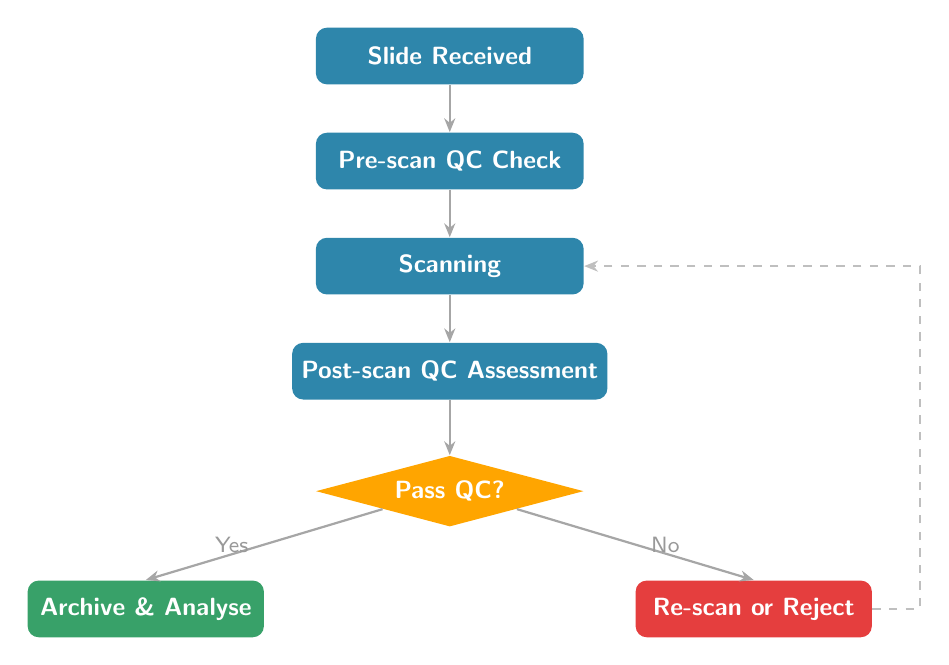
\begin{tikzpicture}[
    node distance = 0.6cm,
    every node/.style = {font=\small\sffamily},
    proc/.style = {
        rectangle, rounded corners=4pt,
        fill={rgb,255:red,46;green,134;blue,171},
        text=white, minimum width=3.4cm, minimum height=0.72cm,
        align=center, font=\small\sffamily\bfseries
    },
    decision/.style = {
        diamond, aspect=2.6,
        fill={rgb,255:red,255;green,165;blue,0},
        text=white, minimum width=3.4cm, minimum height=0.9cm,
        align=center, font=\small\sffamily\bfseries,
        inner sep=1pt
    },
    pass/.style = {
        rectangle, rounded corners=4pt,
        fill={rgb,255:red,56;green,161;blue,105},
        text=white, minimum width=3.0cm, minimum height=0.72cm,
        align=center, font=\small\sffamily\bfseries
    },
    fail/.style = {
        rectangle, rounded corners=4pt,
        fill={rgb,255:red,229;green,62;blue,62},
        text=white, minimum width=3.0cm, minimum height=0.72cm,
        align=center, font=\small\sffamily\bfseries
    },
    arr/.style = {
        -{Stealth[length=5pt,width=4pt]},
        line width=0.8pt, color=gray!70
    },
    lbl/.style = {font=\footnotesize\sffamily, text=gray!80}
]

%% Main vertical chain
\node[proc]     (recv)     {Slide Received};
\node[proc,     below=0.6cm of recv]     (prescan)  {Pre-scan QC Check};
\node[proc,     below=0.6cm of prescan]  (scan)     {Scanning};
\node[proc,     below=0.6cm of scan]     (postscan) {Post-scan QC Assessment};
\node[decision, below=0.7cm of postscan] (decide)   {Pass QC?};

%% Outcome nodes
\node[pass, below left=0.9cm and 1.5cm of decide]  (archive) {Archive \& Analyse};
\node[fail, below right=0.9cm and 1.5cm of decide] (rescan)  {Re-scan or Reject};

%% Arrows — main chain
\draw[arr] (recv)     -- (prescan);
\draw[arr] (prescan)  -- (scan);
\draw[arr] (scan)     -- (postscan);
\draw[arr] (postscan) -- (decide);

%% Arrows — decision branches
\draw[arr] (decide.south west) -- (archive.north)
    node[lbl, midway, left=2pt] {Yes};
\draw[arr] (decide.south east) -- (rescan.north)
    node[lbl, midway, right=2pt] {No};

%% Loop-back dashed arrow for Re-scan
\draw[arr, dashed, color=gray!50]
    (rescan.east) -- ++(0.6,0) |- (scan.east);

\end{tikzpicture}

    \caption{Panoramica del flusso di lavoro per il controllo qualità nella patologia digitale.
    I vetrini progrediscono dall'ispezione pre-scansione attraverso la scansione e il CQ
    post-scansione automatizzato (HistoQC). I vetrini che superano tutti i criteri di CQ vengono
    rilasciati per la refertazione diagnostica o l'analisi computazionale. I vetrini che non
    superano il CQ vengono indirizzati attraverso un percorso di rimedio (nuova scansione, nuova
    colorazione o nuovo montaggio) prima di rientrare nella pipeline di CQ. Le scansioni non
    conformi che non possono essere remediate vengono documentate e segnalate al patologo
    responsabile.}
    \label{fig:qc_workflow}
\end{figure}

% ─────────────────────────────────────────────────────────────
\section{Normalizzazione della Colorazione e Standardizzazione Cromatica}
\label{sec:ch2-normalisation}

\subsection{Fonti di Variabilità della Colorazione}

La variabilità della colorazione è una delle sfide più pervasive nella patologia digitale, che
influenza sia l'interpretazione umana sia l'analisi computazionale. Anche all'interno di un
singolo laboratorio, l'intensità della colorazione e il bilanciamento cromatico possono variare
tra lotti di reagenti, tra corse di colorazione e nel tempo con l'invecchiamento dei reagenti.
Tra laboratori diversi, la variabilità è amplificata dalle differenze nei protocolli di
colorazione, nei fornitori di reagenti, nelle piattaforme di colorazione automatizzata e nelle
pratiche locali. Quando i vetrini vengono scansionati su modelli di scanner diversi o persino su
unità diverse dello stesso modello, viene introdotta un'ulteriore variabilità cromatica dovuta
alle differenze negli spettri di illuminazione, nei sensori della fotocamera e nella calibrazione
cromatica. L'effetto cumulativo è che lo stesso tessuto, colorato e scansionato in due laboratori
diversi, può produrre immagini con caratteristiche cromatiche sostanzialmente diverse, anche se
la biologia sottostante è identica \cite{tellez2019}.

Questa variabilità ha importanti conseguenze pratiche. Per gli osservatori umani, significa che i
patologi devono ricalibrare mentalmente la loro percezione cromatica quando esaminano vetrini di
laboratori non familiari. Per gli algoritmi di IA, significa che un modello addestrato su vetrini
di un laboratorio può avere prestazioni scarse quando applicato a vetrini di un altro, un
fenomeno noto come \emph{domain shift}. La normalizzazione della colorazione --- la trasformazione
computazionale dei colori del vetrino verso uno standard di riferimento comune --- è la strategia
principale per affrontare questo problema \cite{tellez2019}.

\subsection{Deconvoluzione Cromatica: Il Metodo di Ruifrok e Johnston}

La deconvoluzione cromatica è una tecnica matematica per separare i contributi dei singoli
coloranti al colore di ogni pixel in un'immagine E\&E. Il metodo, descritto da Ruifrok e Johnston
\cite{ruifrok2001}, si basa sulla legge di Beer-Lambert dell'assorbimento ottico. Ogni colorante
assorbe la luce a lunghezze d'onda caratteristiche, e il colore osservato di un pixel è il
risultato dell'assorbimento combinato di tutti i coloranti presenti. Se gli spettri di
assorbimento (vettori di colorante) dei singoli coloranti sono noti, il contributo di ciascun
colorante a ogni pixel può essere calcolato risolvendo un sistema di equazioni lineari.

In pratica, i vettori di colorante per l'ematossilina e l'eosina vengono determinati
empiricamente da immagini di riferimento o dalla letteratura. L'algoritmo di deconvoluzione
cromatica trasforma l'immagine RGB in una rappresentazione separata per colorante, producendo
immagini separate per il canale dell'ematossilina (colorazione nucleare) e per il canale
dell'eosina (colorazione citoplasmatica). Il metodo di Ruifrok e Johnston è stato implementato in
piattaforme di analisi delle immagini ampiamente utilizzate, tra cui ImageJ/Fiji e QuPath
\cite{bankhead2017}.

La formulazione matematica della deconvoluzione cromatica è la seguente. Sia $\mathbf{I}$
l'immagine RGB e $\mathbf{M}$ la matrice di colorante $3 \times 3$ le cui colonne sono i vettori
di colorante (spettri di densità ottica) dei singoli coloranti. L'immagine di densità ottica
$\mathbf{OD} = -\log_{10}(\mathbf{I}/\mathbf{I}_0)$, dove $\mathbf{I}_0$ è l'intensità dello
sfondo, può essere decomposta come $\mathbf{OD} = \mathbf{M} \cdot \mathbf{C}$, dove
$\mathbf{C}$ è la matrice delle concentrazioni di colorante. Le concentrazioni di colorante
vengono recuperate con $\mathbf{C} = \mathbf{M}^{-1} \cdot \mathbf{OD}$ \cite{ruifrok2001}.

\subsection{Algoritmi di Normalizzazione della Colorazione}

Gli algoritmi di normalizzazione della colorazione trasformano la distribuzione cromatica di
un'immagine sorgente per farla corrispondere a quella di un'immagine di riferimento (target),
riducendo così la variabilità cromatica inter-vetrino. I metodi classici più utilizzati sono:

\begin{itemize}
    \item \textbf{Normalizzazione di Macenko:} Questo metodo stima la matrice di colorante
    dell'immagine sorgente mediante decomposizione ai valori singolari (SVD) della matrice di
    densità ottica, quindi riscala le concentrazioni di colorante per farle corrispondere a quelle
    dell'immagine di riferimento.

    \item \textbf{Normalizzazione di Vahadane:} Questo metodo utilizza la fattorizzazione a
    matrice non negativa sparsa (SNMF) per stimare la matrice di colorante, più robusta agli
    outlier e più accurata nella separazione dei coloranti rispetto ai metodi basati su SVD.

    \item \textbf{Normalizzazione di Reinhard:} Questo metodo trasferisce le statistiche
    cromatiche (media e deviazione standard) dell'immagine di riferimento all'immagine sorgente
    nello spazio colore LAB. È il metodo di normalizzazione più semplice e veloce.
\end{itemize}

Gli approcci di apprendimento profondo alla normalizzazione della colorazione, incluse le reti
generative avversariali (GAN) e le CycleGAN, hanno dimostrato di produrre immagini normalizzate
visivamente più realistiche rispetto ai metodi classici, ma richiedono grandi dataset di
addestramento e sono computazionalmente costosi \cite{tellez2019}.

\subsection{Importanza per le Applicazioni di IA}

L'importanza della normalizzazione della colorazione per le applicazioni di IA non può essere
sopravvalutata. I modelli di apprendimento profondo per la patologia computazionale vengono
addestrati su grandi dataset di WSI annotate, e le loro prestazioni sono altamente sensibili alle
caratteristiche cromatiche dei dati di addestramento. La normalizzazione della colorazione,
applicata in modo coerente sia ai dati di addestramento sia a quelli di test, riduce questo
\emph{domain shift} indotto dal colore e migliora la generalizzabilità dei modelli di IA tra
laboratori e scanner \cite{tellez2019}.

% ─────────────────────────────────────────────────────────────
\section{Collaborazione tra Tecnico e Patologo}
\label{sec:ch2-collaboration}

\subsection{Ruoli Complementari}

Il laboratorio di patologia digitale è un ambiente collaborativo in cui i tecnici di laboratorio
e i patologi svolgono ruoli complementari e interdipendenti. I tecnici sono responsabili della
preparazione fisica dei vetrini --- fissazione, processazione, inclusione, sezionamento,
colorazione e coprioggetto --- e del funzionamento delle apparecchiature di scansione. Sono la
prima linea del controllo qualità, eseguendo l'ispezione visiva dei vetrini prima della
scansione e monitorando la qualità della scansione in tempo reale. I patologi sono responsabili
dell'interpretazione diagnostica delle immagini digitali e dell'accettazione o del rifiuto finale
delle immagini come idonee alla diagnosi.

La transizione alla patologia digitale ha, per certi versi, aumentato l'importanza del ruolo del
tecnico. Nella patologia tradizionale su vetrino, il patologo può compensare le carenze minori
nella preparazione del vetrino regolando la messa a fuoco o l'illuminazione del microscopio.
Nella patologia digitale, il patologo dipende interamente dalla qualità dell'immagine scansionata;
non c'è possibilità di riesaminare il vetrino fisico durante la sessione diagnostica. Ciò pone
un onere maggiore sul tecnico per garantire che i vetrini siano della massima qualità possibile
prima della scansione.

\subsection{Flusso di Comunicazione e Segnalazione dei Problemi di Qualità}

Il flusso di comunicazione in un laboratorio di patologia digitale segue tipicamente un percorso
strutturato. Quando un tecnico identifica un problema di qualità --- ad esempio, un vetrino con
una piega tissutale, una bolla d'aria o un artefatto di colorazione --- segnala il problema nel
SIL e, se necessario, contatta direttamente il patologo responsabile. La segnalazione deve
includere una descrizione del problema, i vetrini interessati e la valutazione del tecnico sulla
probabilità che il problema influenzi l'interpretazione diagnostica.

Gli strumenti di CQ automatizzati come HistoQC \cite{janowczyk2019} possono pre-filtrare i
vetrini e indirizzare solo quelli con problemi di qualità significativi alla revisione umana,
riducendo il carico sia sui tecnici sia sui patologi. Tuttavia, gli strumenti automatizzati non
possono sostituire il giudizio umano per i casi limite, e la decisione finale sull'idoneità
diagnostica di un vetrino deve sempre spettare al patologo responsabile.

\subsection{Procedure di Escalation}

Le procedure di escalation definiscono il percorso per la gestione dei problemi di qualità che
non possono essere risolti a livello del tecnico. Un tipico percorso di escalation potrebbe
essere: (1) il tecnico identifica il problema di qualità e tenta la rimediazione (ad es., nuova
scansione, nuovo montaggio); (2) se la rimediazione non ha successo, il tecnico segnala il
problema al biologo senior o al responsabile del laboratorio; (3) se il problema non può essere
risolto a livello del biologo senior, viene escalato al patologo responsabile; (4) se il patologo
determina che il problema di qualità influisce sull'interpretazione diagnostica e non può essere
risolto, il caso viene escalato al team clinico con un referto che indica la limitazione di
qualità.

\subsection{Standard di Documentazione}

La documentazione è la spina dorsale della gestione della qualità nel laboratorio di patologia
digitale. Ogni azione correlata alla qualità --- dall'ispezione visiva pre-scansione alla
decisione del patologo di accettare un'immagine non ottimale --- deve essere registrata in un
formato standardizzato recuperabile per scopi di audit. Gli standard di documentazione devono
specificare: le informazioni da registrare (identificatore del vetrino, data e ora, natura del
problema, azione intrapresa, esito); il formato del registro (inserimento dati strutturato nel
SIL, commento in testo libero o entrambi); e il periodo di conservazione dei registri.

% ─────────────────────────────────────────────────────────────
\section{Documentazione e Tracciabilità}
\label{sec:ch2-documentation}

\subsection{Catena di Custodia}

La catena di custodia si riferisce al registro documentato del possesso, della gestione e della
localizzazione di un campione dal momento della raccolta a quello dello smaltimento. In patologia,
il mantenimento di una catena di custodia ininterrotta è un requisito legale ed etico, poiché
garantisce che il campione esaminato dal patologo sia lo stesso campione prelevato dal paziente.
Nel contesto della patologia digitale, la catena di custodia si estende all'immagine digitale:
l'immagine deve essere dimostrabilmente collegata al vetrino fisico, che deve essere
dimostrabilmente collegato al campione del paziente.

La catena di custodia è mantenuta attraverso una combinazione di etichettatura fisica (codici a
barre, codici QR o tag RFID su contenitori di campioni, cassette e vetrini) e registrazioni
elettroniche nel SIL. Ogni trasferimento di custodia deve essere registrato con un timestamp e
l'identità della persona responsabile. Le conseguenze di un'interruzione della catena di custodia
possono essere gravi: un campione etichettato in modo errato o confuso con un altro campione può
portare a una diagnosi errata, con conseguenze potenzialmente catastrofiche per il paziente.

\subsection{Codici a Barre e Identificazione Digitale}

Il codice a barre è la tecnologia principale per l'identificazione dei campioni nel moderno
laboratorio di patologia. I codici a barre vengono stampati su contenitori di campioni, cassette
e vetrini al momento dell'etichettatura, e vengono letti in ogni fase del flusso di lavoro per
verificare l'identità del campione e registrare il trasferimento di custodia. I codici a barre
bidimensionali (codici QR, codici DataMatrix) sono preferiti a quelli unidimensionali perché
possono codificare più informazioni in uno spazio più piccolo e sono più resistenti ai danni.

Nel flusso di lavoro della patologia digitale, il codice a barre del vetrino viene letto dallo
scanner al momento del caricamento, e l'immagine digitale risultante viene automaticamente
collegata al corrispondente registro del caso nel SIL. Questo collegamento automatizzato elimina
il rischio di errori di trascrizione manuale.

\subsection{Audit Trail Digitali}

Un audit trail digitale è un registro cronologico di tutte le azioni eseguite su un oggetto
digitale --- in questo contesto, un file WSI. L'audit trail registra chi ha avuto accesso
all'immagine, quando, da quale dispositivo e quale azione è stata intrapresa (visualizzazione,
annotazione, refertazione, esportazione, eliminazione). Gli audit trail digitali sono essenziali
per la conformità normativa, per scopi medicolegali e per l'indagine di incidenti di qualità.

\subsection{Requisiti Normativi}

I laboratori di patologia digitale sono soggetti a una serie di requisiti normativi e di
accreditamento che disciplinano la qualità dei loro processi e della loro documentazione. Gli
standard più rilevanti sono:

\begin{itemize}
    \item \textbf{ISO 15189:} Lo standard internazionale per i laboratori medici, ISO 15189
    specifica i requisiti per la qualità e la competenza nei test di laboratorio medico. Richiede
    ai laboratori di stabilire e mantenere un sistema di gestione della qualità, di validare i
    propri metodi analitici, di partecipare a programmi di valutazione esterna della qualità (VEQ)
    e di mantenere una documentazione completa di tutte le attività correlate alla qualità.

    \item \textbf{Accreditamento CAP:} Il College of American Pathologists (CAP) Laboratory
    Accreditation Program fornisce l'accreditamento per i laboratori di patologia negli Stati
    Uniti e a livello internazionale. Il CAP ha pubblicato liste di controllo specifiche per la
    patologia digitale, che coprono la validazione dello scanner, la gestione delle immagini, le
    procedure di CQ e la refertazione diagnostica.

    \item \textbf{IVDR (UE):} Nell'Unione Europea, i sistemi di patologia digitale utilizzati per
    la diagnosi primaria sono regolamentati come dispositivi medici diagnostici in vitro (IVD) ai
    sensi del Regolamento sui Dispositivi Medico-Diagnostici In Vitro (IVDR, UE 2017/746).
\end{itemize}

% ─────────────────────────────────────────────────────────────
\section{Attività Pratiche}
\label{sec:ch2-practical}

\subsection{Attività A: Esercizio di Riconoscimento degli Artefatti}

\textbf{Obiettivo:} Sviluppare la capacità di identificare e classificare gli artefatti comuni
nelle immagini di patologia digitale e valutare il loro impatto sulla qualità diagnostica.

\textbf{Materiali:} Un set curato di 20 immagini di vetrini interi (o tessere di immagine
rappresentative) tratte da un dataset pubblicamente disponibile (ad es., TCGA) o dall'archivio
del laboratorio, inclusi esempi dei seguenti artefatti: bolle d'aria, pieghe tissutali, regioni
sfocate, polvere e detriti, segni di penna e difetti del coprioggetto. Deve essere fornita una
guida di riferimento per la classificazione degli artefatti.

\textbf{Procedura:}
\begin{enumerate}
    \item Gli studenti esaminano ogni immagine in modo indipendente e registrano la loro
    valutazione di: (a) il tipo/i di artefatto presente; (b) la proporzione dell'area tissutale
    interessata; (c) se l'artefatto è probabile che influenzi l'interpretazione diagnostica; e
    (d) l'azione di rimediazione raccomandata (nuova scansione, nuova colorazione, nuovo montaggio
    o accettazione con annotazione).

    \item Gli studenti confrontano le loro valutazioni con quelle di un patologo di riferimento
    (fornite come chiave delle risposte) e calcolano il loro tasso di accordo per ogni categoria
    di artefatto.

    \item In piccoli gruppi, gli studenti discutono i casi in cui la loro valutazione differiva
    da quella di riferimento e identificano le ragioni del disaccordo.

    \item Gli studenti utilizzano la pipeline HistoQC \cite{janowczyk2019} per eseguire il CQ
    automatizzato su un sottoinsieme delle immagini e confrontano i risultati del CQ automatizzato
    con le loro valutazioni manuali.
\end{enumerate}

\textbf{Risultati di apprendimento:} Al termine di questa attività, gli studenti dovrebbero
essere in grado di identificare e classificare i principali tipi di artefatti nelle immagini di
patologia digitale, valutarne la rilevanza diagnostica e applicare strumenti di CQ automatizzati
a supporto della valutazione della qualità.

\subsection{Attività B: Studio di Caso --- Flusso di Lavoro Digitale dalla Biopsia alla Diagnosi}

\textbf{Obiettivo:} Tracciare il flusso di lavoro completo della patologia digitale per un caso
clinico, dalla ricezione del campione alla refertazione diagnostica, identificando i punti di
controllo qualità e i potenziali punti di errore in ogni fase.

\textbf{Materiali:} Un caso clinico anonimizzato (fornito dal coordinatore del corso) che include:
il modulo di richiesta, la descrizione macroscopica, le immagini WSI delle sezioni istologiche
(E\&E e IIC), i risultati del CQ automatizzato da HistoQC e il referto diagnostico finale.

\textbf{Procedura:}
\begin{enumerate}
    \item Gli studenti esaminano il caso clinico e costruiscono una mappa del flusso di lavoro
    che tracci il percorso del campione dalla ricezione alla diagnosi, identificando ogni fase,
    il personale responsabile e i criteri di qualità applicabili.

    \item Gli studenti esaminano i risultati del CQ di HistoQC e identificano eventuali problemi
    di qualità nelle immagini WSI. Per ogni problema identificato, propongono un'azione di
    rimediazione e valutano l'impatto potenziale sulla diagnosi.

    \item Gli studenti esaminano le immagini WSI in QuPath e confrontano le loro osservazioni
    diagnostiche con il referto finale. Identificano le caratteristiche morfologiche chiave che
    supportano la diagnosi e valutano se eventuali problemi di qualità dell'immagine hanno
    influenzato la loro capacità di identificare queste caratteristiche.

    \item Gli studenti redigono un breve rapporto (circa 500 parole) che descrive il flusso di
    lavoro del caso, i problemi di qualità identificati, le azioni di rimediazione proposte e
    le lezioni apprese per la pratica futura.
\end{enumerate}

\textbf{Risultati di apprendimento:} Al termine di questa attività, gli studenti dovrebbero
essere in grado di tracciare il flusso di lavoro completo della patologia digitale per un caso
clinico, identificare i punti di controllo qualità e i potenziali punti di errore, e applicare
strumenti di CQ automatizzati e manuali per valutare la qualità dell'immagine.

% ─────────────────────────────────────────────────────────────
\section{Riepilogo}
\label{sec:ch2-summary}

Questo capitolo ha esaminato il flusso di lavoro della patologia digitale e il controllo qualità,
dalla preparazione del campione all'immagine archiviata. I seguenti punti chiave devono essere
ricordati:

\begin{itemize}
    \item Il flusso di lavoro della patologia digitale è una pipeline lineare con diverse fasi
    discrete, ognuna delle quali introduce potenziali fonti di variabilità ed errore. Il controllo
    qualità deve operare a ogni fase per garantire l'integrità diagnostica.

    \item I fattori pre-analitici --- fissazione, processazione, sezionamento, colorazione e
    coprioggetto --- esercitano la maggiore influenza sulla qualità finale dell'immagine e non
    possono essere corretti computazionalmente dopo la scansione.

    \item La valutazione della qualità della messa a fuoco, dell'uniformità della colorazione e
    degli artefatti è essenziale per garantire che le immagini siano idonee alla diagnosi e
    all'analisi computazionale. Strumenti automatizzati come HistoQC \cite{janowczyk2019}
    supportano ma non sostituiscono il giudizio umano.

    \item La normalizzazione della colorazione --- mediante metodi come Macenko, Vahadane o
    Reinhard --- riduce la variabilità cromatica inter-laboratorio e migliora la
    generalizzabilità dei modelli di IA \cite{tellez2019}. La deconvoluzione cromatica secondo
    Ruifrok e Johnston \cite{ruifrok2001} consente l'analisi quantitativa dei singoli coloranti.

    \item La collaborazione tra tecnico e patologo è fondamentale per un servizio di patologia
    digitale di alta qualità. I tecnici sono la prima linea del controllo qualità; i patologi
    sono responsabili dell'accettazione finale delle immagini come idonee alla diagnosi.

    \item La documentazione e la tracciabilità --- incluse la catena di custodia, i codici a
    barre, gli audit trail digitali e la conformità agli standard normativi (ISO 15189, CAP,
    IVDR) --- sono requisiti non negoziabili per un servizio di patologia digitale clinicamente
    sicuro e legalmente conforme.
\end{itemize}

% ─────────────────────────────────────────────────────────────
\section{Domande di Revisione}
\label{sec:ch2-questions}

\begin{enumerate}

    \item \label{ch2:q1} Quale fissativo è più comunemente utilizzato per la processazione
    tissutale istologica di routine nella patologia digitale?
    \begin{enumerate}[label=\Alph*.]
        \item Alcool etilico al 70\%
        \item Glutaraldeide al 2,5\%
        \item Formalina neutra tamponata al 10\%
        \item Soluzione di Bouin
    \end{enumerate}

    \item \label{ch2:q2} Qual è lo scopo principale della normalizzazione della colorazione nella
    patologia digitale?
    \begin{enumerate}[label=\Alph*.]
        \item Aumentare la risoluzione delle immagini WSI
        \item Ridurre la variazione nell'aspetto della colorazione causata da laboratori,
        protocolli e scanner diversi
        \item Eliminare la necessità di colorazione IIC
        \item Convertire le immagini a colori in immagini in scala di grigi per l'analisi
    \end{enumerate}

    \item \label{ch2:q3} Quale dei seguenti artefatti è più probabile che causi una regione di
    un'immagine di vetrino intero che appare sfocata?
    \begin{enumerate}[label=\Alph*.]
        \item Sovra-colorazione con ematossilina
        \item Contaminazione batterica del campione
        \item Spessore tissutale non uniforme
        \item Uso di un obiettivo a basso ingrandimento
    \end{enumerate}

    \item \label{ch2:q4} Il metodo di deconvoluzione cromatica sviluppato da Ruifrok e Johnston
    viene utilizzato per:
    \begin{enumerate}[label=\Alph*.]
        \item Aumentare la risoluzione delle immagini WSI mediante interpolazione
        \item Separare i contributi dei singoli coloranti (ad es., ematossilina e DAB) da
        un'immagine RGB
        \item Convertire le immagini WSI dal formato SVS al formato OME-TIFF
        \item Rilevare automaticamente le regioni tumorali nelle immagini WSI
    \end{enumerate}

    \item \label{ch2:q5} Nel contesto del controllo qualità nella patologia digitale, HistoQC è:
    \begin{enumerate}[label=\Alph*.]
        \item Un sistema commerciale di gestione delle immagini per la patologia digitale
        \item Uno strumento open source per la valutazione automatizzata della qualità delle
        immagini di vetrini interi
        \item Un protocollo di colorazione standardizzato per l'E\&E
        \item Un formato di file per l'archiviazione di immagini WSI
    \end{enumerate}

    \item \label{ch2:q6} Quale dei seguenti descrive meglio la fase pre-analitica nella patologia
    digitale?
    \begin{enumerate}[label=\Alph*.]
        \item Solo la fase di scansione del vetrino
        \item Solo la fase di refertazione diagnostica
        \item Tutte le fasi dalla ricezione del campione alla scansione del vetrino
        \item Solo la fase di analisi computazionale dell'immagine
    \end{enumerate}

    \item \label{ch2:q7} Qual è il motivo principale per cui il tempo di fissazione deve essere
    attentamente controllato nella patologia digitale?
    \begin{enumerate}[label=\Alph*.]
        \item Il tempo di fissazione influenza la dimensione del file WSI
        \item Il tempo di fissazione influenza la morfologia tissutale, la preservazione degli
        antigeni e le analisi IIC e molecolari successive
        \item Il tempo di fissazione determina il numero di livelli della piramide di immagine
        \item Il tempo di fissazione influenza la velocità di scansione dello scanner
    \end{enumerate}

    \item \label{ch2:q8} Quale dei seguenti è il primo passo più appropriato quando si scopre che
    una WSI scansionata presenta significative regioni sfocate?
    \begin{enumerate}[label=\Alph*.]
        \item Accettare l'immagine con un'annotazione di qualità e procedere con la diagnosi
        \item Eliminare l'immagine e richiedere un nuovo campione al chirurgo
        \item Riscansionare il vetrino dopo aver verificato la calibrazione della messa a fuoco
        dello scanner
        \item Applicare un filtro di nitidezza computazionale all'immagine
    \end{enumerate}

    \item \label{ch2:q9} In un laboratorio di patologia digitale, la documentazione della catena
    di custodia serve a:
    \begin{enumerate}[label=\Alph*.]
        \item Ridurre il tempo di scansione dei vetrini
        \item Garantire la tracciabilità dei campioni e dei vetrini attraverso il flusso di lavoro
        \item Migliorare la qualità della colorazione E\&E
        \item Aumentare la velocità di refertazione diagnostica
    \end{enumerate}

    \item \label{ch2:q10} Quale standard internazionale è più rilevante per la gestione della
    qualità in un laboratorio medico che esegue patologia digitale?
    \begin{enumerate}[label=\Alph*.]
        \item ISO 9001
        \item ISO 15189
        \item ISO 27001
        \item ISO 13485
    \end{enumerate}

\end{enumerate}
